\documentclass[10pt,a4paper]{article}
\usepackage[latin1]{inputenc}
\usepackage{amsmath}
\usepackage{amsfonts}
\usepackage{amssymb}
\usepackage{graphicx}
\usepackage{float}
\usepackage{soul}
\usepackage{caption}
\usepackage{subcaption}
\usepackage[section]{placeins}
\usepackage[left=2cm,right=2cm,top=2cm,bottom=2cm]{geometry}
\author{Akshat Mahajan}
\title{Physics 180Q - Lab Report 6}
\begin{document}
\maketitle
\noindent \textsl{This lab was performed in conjunction with Hanwen Qin. Variable impedance terminator resistance for photodiode was 10 kilo-Ohms.}
\section*{Part 1: Measuring Threshold Current and Laser Spectrum}
In this section, we measured various properties of our laser diode. Laser diodes have a spectrum dependent on temperature as well as current - at a certain threshold current, the power of the laser sharply increases to reach a maximum beyond that voltage. We used a 633 nm laser beam.\\
\\
The equipment involved used a temperature and current controller for the laser diode. The current controller registers currents internally in milli-amperes (mA), whereas the temperature controller uses resistance values in kilo-Ohms (k$\Omega$) and a conversion equation 
$$ R = R_{0}\exp{\left[\beta\left(\dfrac{1}{T} - \dfrac{1}{T_{0}}\right)\right]}$$
where $\beta = 3977$ K, $T_{0}$ is our reference temperature of 298 K, and $R_{0}$ our reference resistance value of 10 k$\Omega$ at 298 K.\\
\\
We first measured the threshold current in two different ways at a laser temperature of 298 K:
\begin{itemize}
\item \textbf{By eye} - We varied the knob on the current controller while aiming the laser at a piece of paper. A sharp and sudden spike was observed at about \textbf{17.77} mA.
\item \textbf{By plot} - This was the more complicated method. We began by connecting the output and input terminals of the temperature controller to an oscilloscope and sawtooth generator respectively, and 'driving' the current at a peak-to-peak amplitude of 75 mV\footnote{Please see the conversion equation from driving voltage to current.}, at a frequency of 1 Hz. The initial current reading on the current controller was 18.06 mA, and was taken to be the true offset. The equation needed to convert applied voltage to current reading is as follows:
$$ I_{\mathrm{out}} = I_{\mathrm{offset}} +\left( \dfrac{I_{\mathrm{max}}}{V_{\mathrm{max}}}\times V_{\mathrm{applied}} \right) = 18.06\;\mathrm{mA} + \left( \dfrac{50\;\mathrm{mA}}{10\;\mathrm{V}}\times V_{\mathrm{applied}} \right)$$
with V$_{\mathrm{applied}}$ in volts and I$_{\mathrm{out}}$ in mA and is the current reading when the generator is turned off. It should be noted that current limits in the laser diode are reached at about 40 mA. Below are figures of our measurements:
\end{itemize}
\begin{figure}[H]
\centering
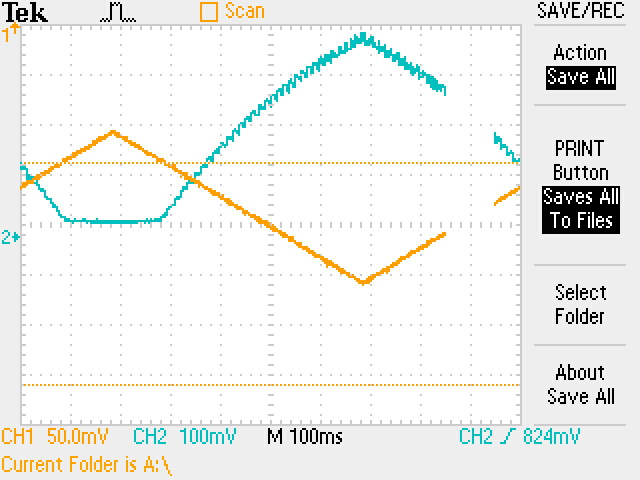
\includegraphics[scale=0.3]{../Analysis/F0003TEK.JPG} 
\caption{Oscilloscope Image for Threshold Current Determination}
\end{figure}
\begin{figure}[H]
\centering
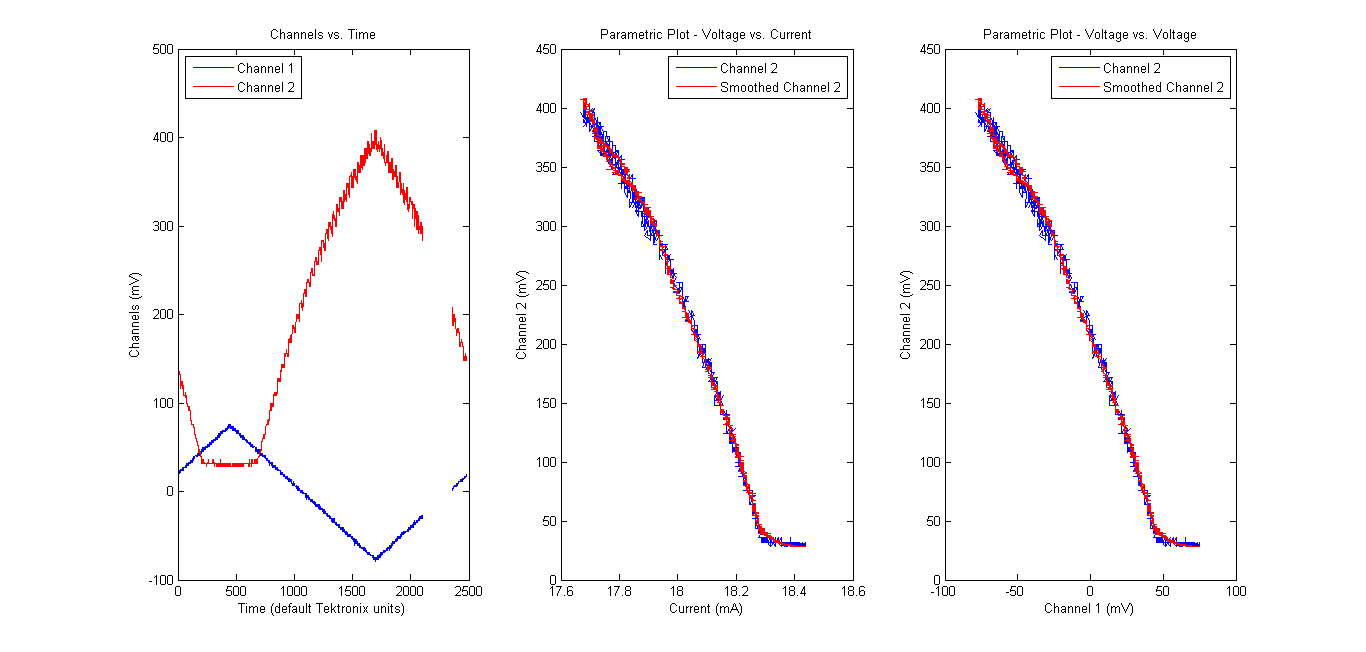
\includegraphics[scale=0.5]{../Analysis/ThresholdCurrentDetF0000.png} 
\caption{Current Determination. Channel 1 corresponds to the output from the sawtooth function generator, and Channel 2 corresponds to the response of the laser diode as a proxy for laser power. (Left) Output from sawtooth generator and laser response over time (Center) A parametric plot of Channel 2 versus current obtained from the conversion equation (Right) A parametric plot of Channel 2 versus Channel 1. Our threshold current can be readily seen to be roughly \textbf{18.3} mA. Channel 2 is smoothened by interpolating between every 100 points in the parametric plots above.}
\end{figure}
\noindent Determining the threshold frequency in the plots of Figures 1 and 2 was in turn accomplished in a couple of ways:
\begin{itemize}
\item \textit{By eye} - We simply chose\footnote{The actual raw data from the oscilloscope for channel 1 includes an important offset from the pictorial data that, when not corrected for, appears to result in a threshold current of approximately 16.8 mA. Evidence for the existence of this offset comes from the fact that parametric plots otherwise do \textsl{not} correspond to sinusoidal oscillations about 18.06 mA.  In this report, I have taken care to correct for this term by subtracting the average value of the reading, so as to faithfullly mimic Figure 1.} the point that appeared closest to the marked steep rise in the data to the human eye. Doing it this way, the result comes out to be around 18.3 mA. This was confirmed by comparison to the parametric plots with the time-dependent plots in Figure 1, as well as by the cursor reading of the oscilloscope.
\item \textit{By computing the point with the maximum rate of change} - Unfortunately, this was foiled by the jagged, non-smooth nature of the curve. An attempt was made to smoothen the curve, but this continued to result in intense jaggedness (as can be seen in the right and center parametric plots of Figure 2). We decided to default to the approach by eye.
\end{itemize}
\begin{table}[H]
\centering
\begin{tabular}{|c|c|}
\hline 
By eye & 17.8 mA \\ 
\hline 
By plot & 18.3 mA \\ 
\hline 
Average & \textbf{18.05} mA\\
\hline
\end{tabular} 
\caption{Threshold currents by measurement method}
\end{table}
We take our threshold current to be 18.05 mA.
\subsection*{Measuring Spectra}
We next measured the spectrum of the laser above and below the threshold current at a constant temperature of 298 K. As an extra item, we chose to do more than one measurement below threshold. From these measurements, we attempted to calculate the cavity length of the laser as well as the resolution of the spectrometer.\\
\\
We chose the following currents for our measurements: 16.61 mA, 16.43 mA and finally 19 mA. The first two fall well below our threshold current of 18.05 mA, whereas the first is significantly above it.\\
\\
To prevent saturation of the spectrometer at 19 mA, a knife edge was used to partially block the laser beam. Figures 3, 4 and 5 document the spectrum behaviour. The intensity is presented in arbitrary units.
\begin{figure}[H]
\centering
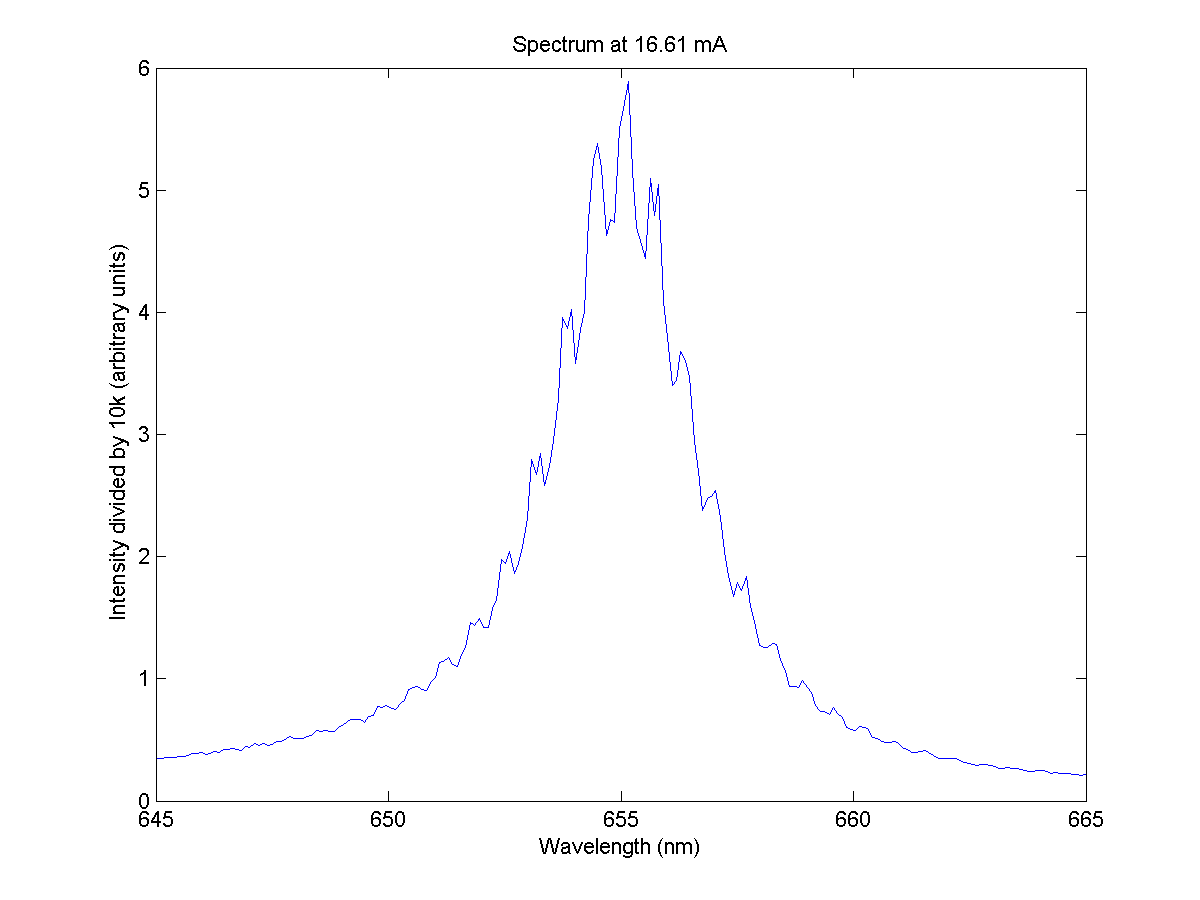
\includegraphics[scale = 0.4]{../Analysis/BelThresh1.png}
\caption{Below Threshold Spectrum Measurements} 
\end{figure} 
\begin{figure}[H]
\centering
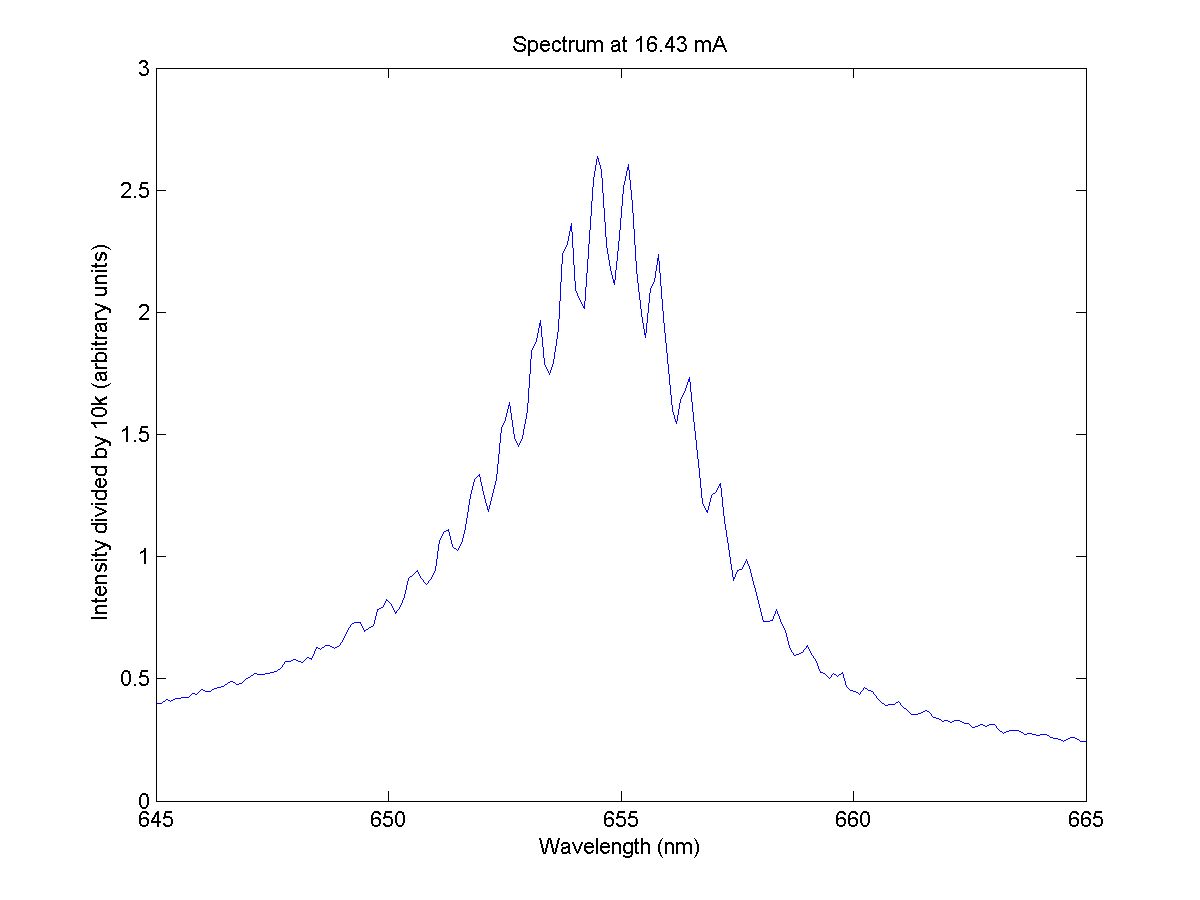
\includegraphics[scale = 0.4]{../Analysis/BelThresh2.png}
\caption{Below Threshold Spectrum Measurements} 
\end{figure} 
\begin{figure}[H]
\centering
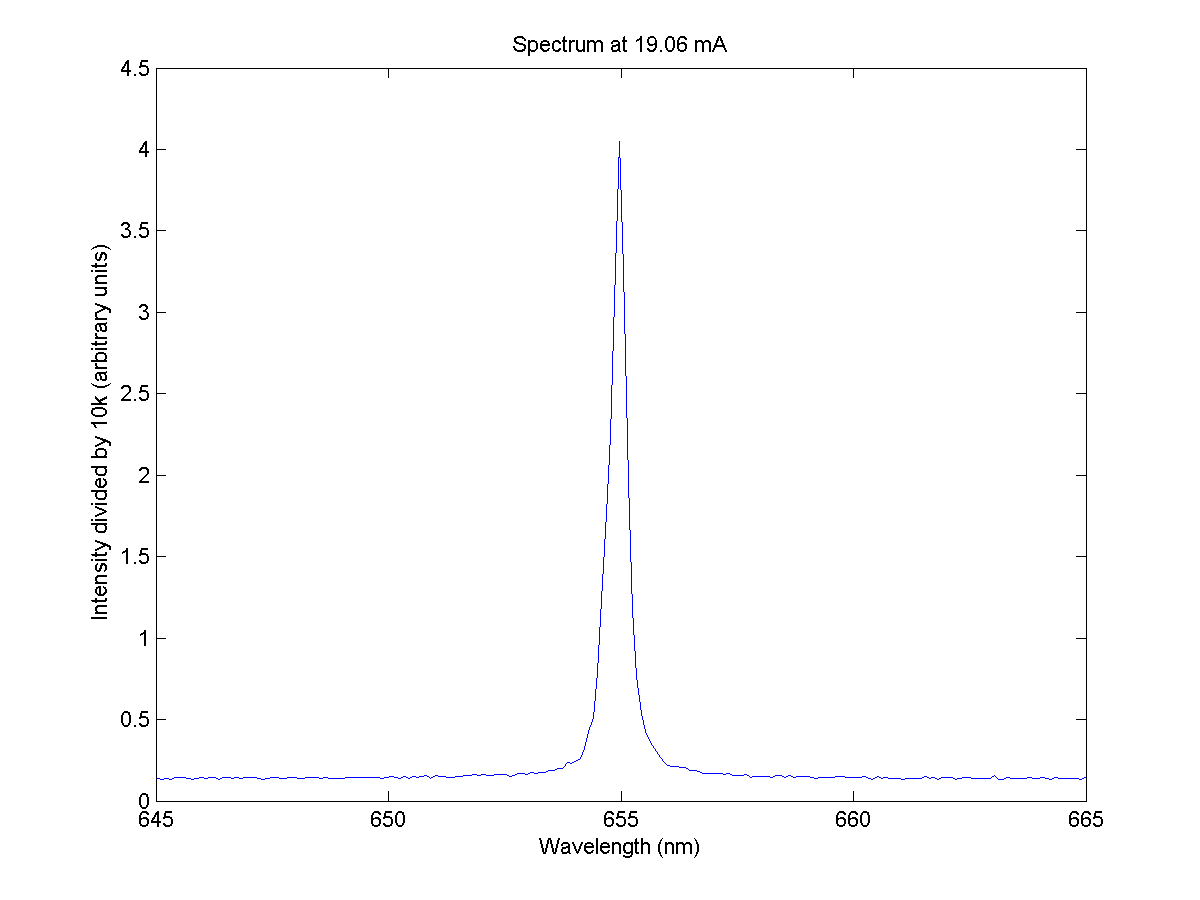
\includegraphics[scale = 0.4]{../Analysis/AboThresh.png}
\caption{Above Threshold Spectrum Measurements} 
\end{figure} 
\noindent We note distribution of mode orders at each current in Table 2. As mentioned in the lab manual, one mode is preferentially selected above threshold, from which we can estimate the full width half maximum (the line spacing).
\begin{table}[H]
\centering
\begin{tabular}{|p{3cm}|p{2cm}|p{2cm}|c|}
\hline
& \multicolumn{3}{c|}{Wavelengths (nm) at Various Currents}
\\
\hline
Currents & 16.61 mA & 16.43 mA & 19.06 mA  \\ 
\hline 
Zero-order modes & 655.2 & 655.2 & 655 \\ 
\hline 
First-order modes & 654.5 \textbf{and} 655.6 & 654.5 \textbf{and} 655.8 & - \\
\hline
Second-order modes & 653.8 \textbf{and} 656.3 & 653.9 \textbf{and} 656.5 & - \\
\hline
\end{tabular} 
\caption{Mode order occurrences in Figures 3, 4 and 5.}
\end{table}
\noindent To calculate cavity length from mode spacings, we employ the following relationship that can be derived for a Fabry-Perot cavity
$$ \Delta \lambda = \dfrac{\lambda^{2}}{2\eta\ell}$$
where $\lambda$ is the laser's operating wavelength (here taken to be 655 nm), $\Delta \lambda$ is our wavelength mode spacing and $\ell$ our cavity width, $\eta$ (we take to be about 3.5) is our diode medium index of refraction, and $\ell$ our cavity spacing. We use the mode spacing between the zero and first order modes for our calculation.
$$ \ell = \dfrac{\lambda^{2}}{2\eta\Delta\lambda} = \dfrac{\left(655^{2} \times 10^{-18}\right)}{2\times 3.5 \times (655.2 - 654.6)} \; \mathrm{m} = \dfrac{429025}{7\times 0.6} \times 10^{-18} \; \mathrm{m} = \mathbf{1.02}\; \mathrm{mm}$$
The small variances between different current mode spacing measurements is not enough to significantly alter the value of this result. For an L650P007 laser diode from Thorlabs (the closest diode which matches our behaviour), this appears to be roughly commensurate with the manufacturer's value of \textbf{1.2 mm}.\\
\\
The linewidth above threshold is essentially the full width half maximum of our laser, and was measured at 19.06 mA (above threshold) as 655.1 - 654.7 nm = \textbf{0.4} nm. This is just the resolution bandwidth (or essentially the free spectral range divided by the finesse of the laser cavity). The smaller this is, the higher the quality factor of the cavity.
\subsection*{Measuring Temperature and Current Dependence}
We took six measurements, three at fixed temperature and three at fixed current to understand the response of the laser to these conditions. At the time of performing this experiment, we luckily avoided laser saturation by consistently taking measurements below the threshold current. Some (but not all) of our chosen data points are plotted below in the following figures.
\begin{figure}[H]
\centering
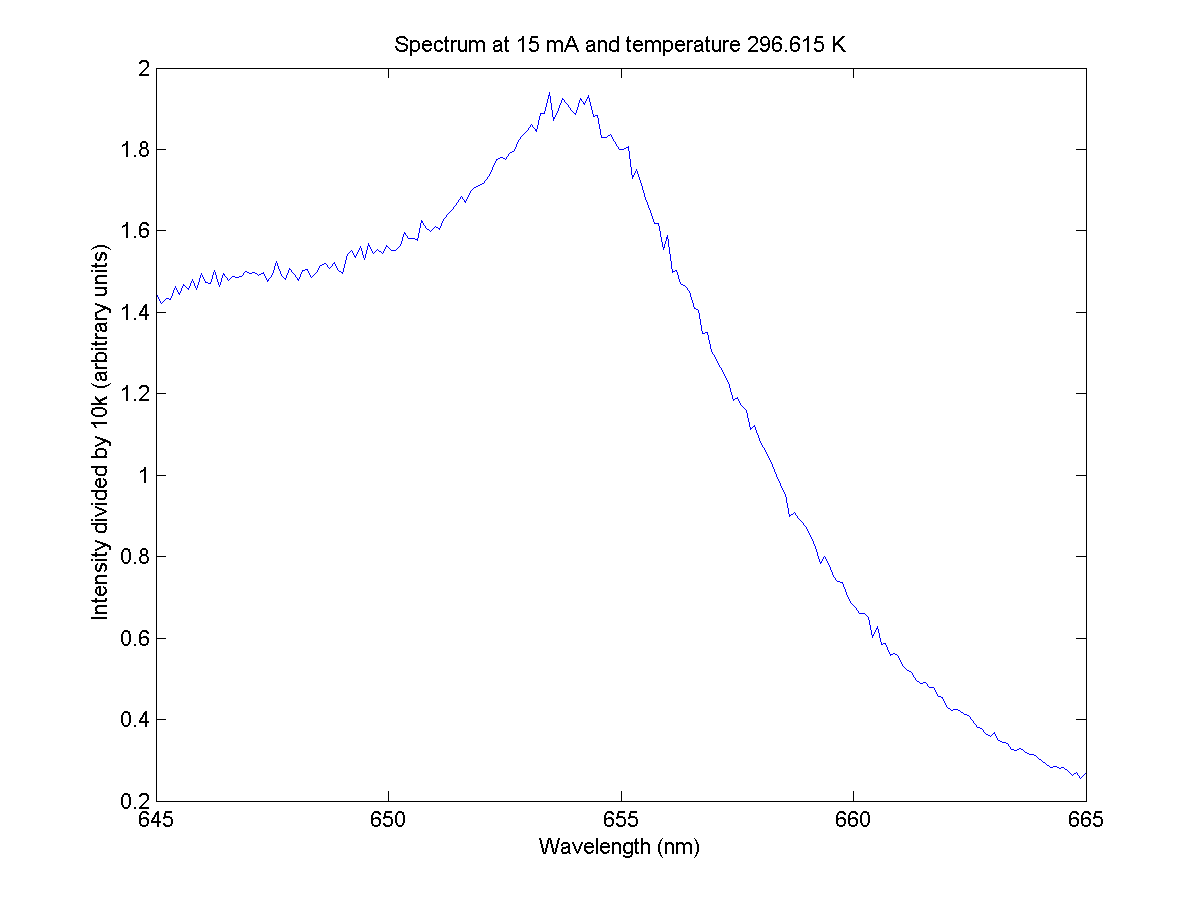
\includegraphics[scale = 0.5]{../Analysis/15mAT10p643.png}
\end{figure} 
\begin{figure}[H]
\centering
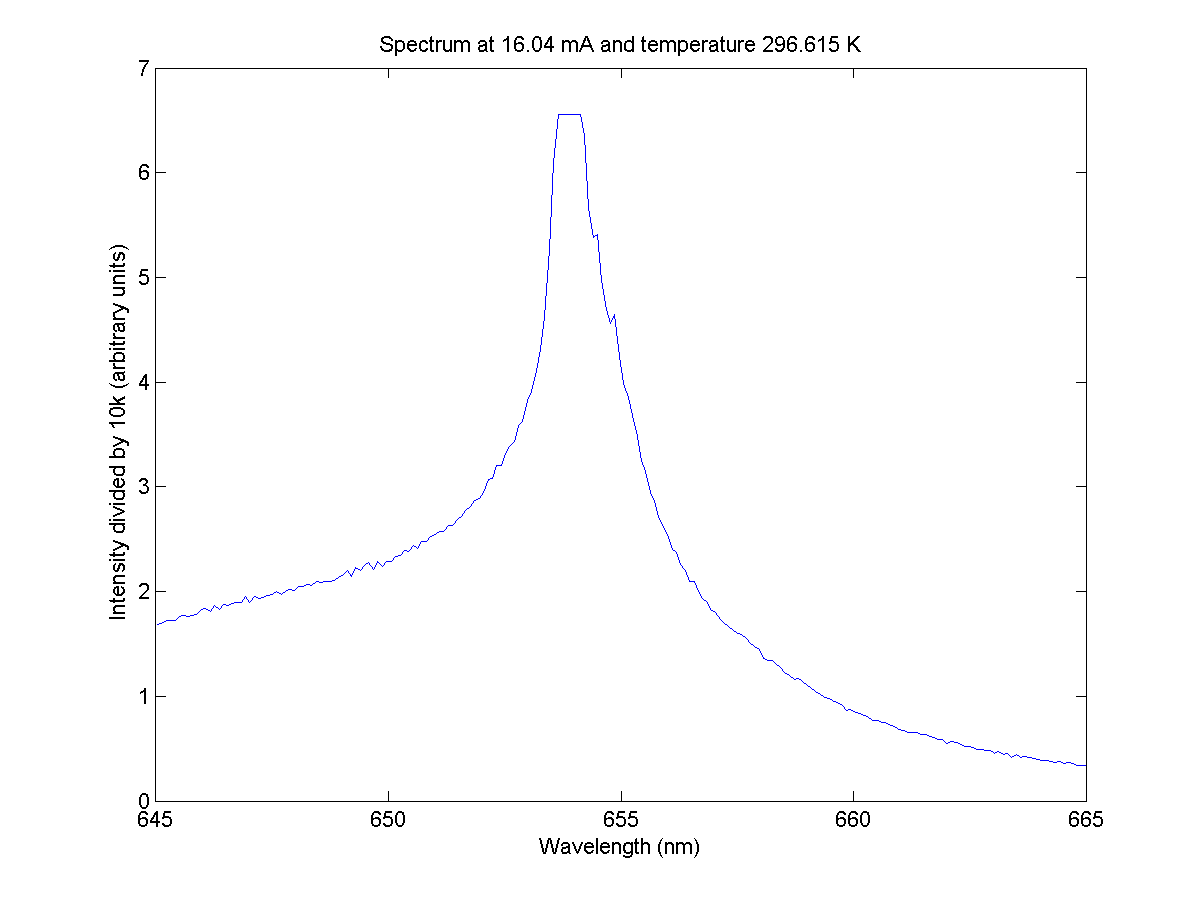
\includegraphics[scale = 0.5]{../Analysis/16p04mAT10p643.png}
\end{figure} 
\begin{figure}[H]
\centering
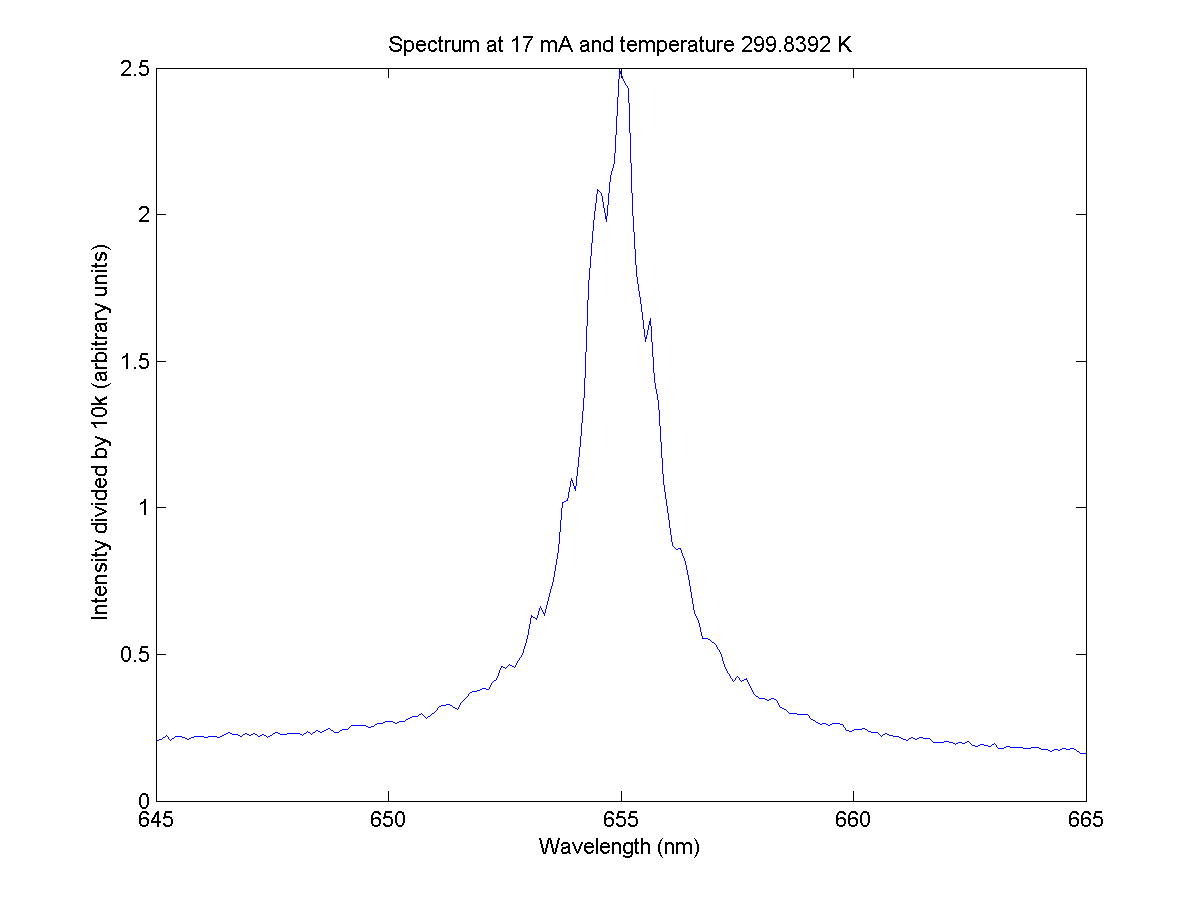
\includegraphics[scale = 0.5]{../Analysis/17mAT9p214.png} 
\end{figure}
\begin{figure}[H]
\centering
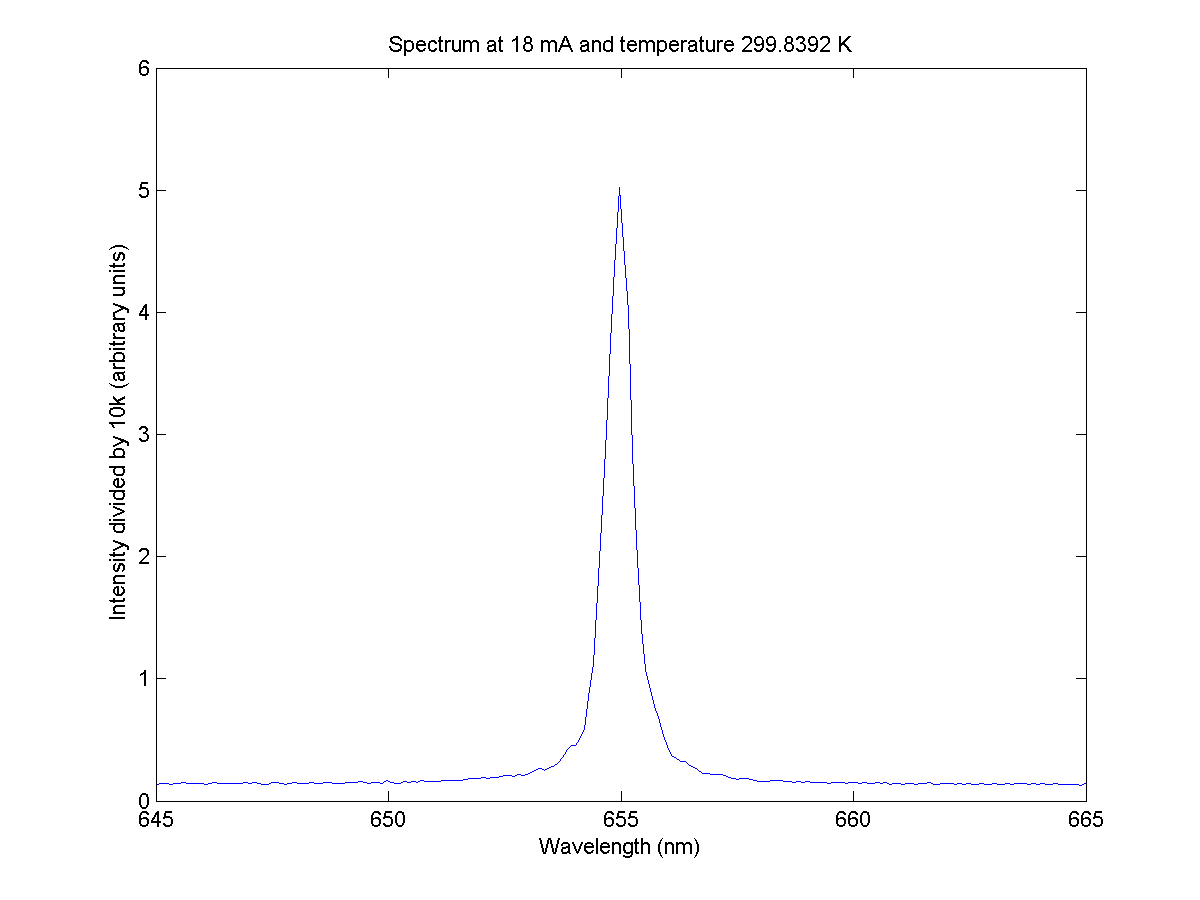
\includegraphics[scale = 0.5]{../Analysis/18mAT9p214.png}
\end{figure} 
\begin{figure}[H]
\centering
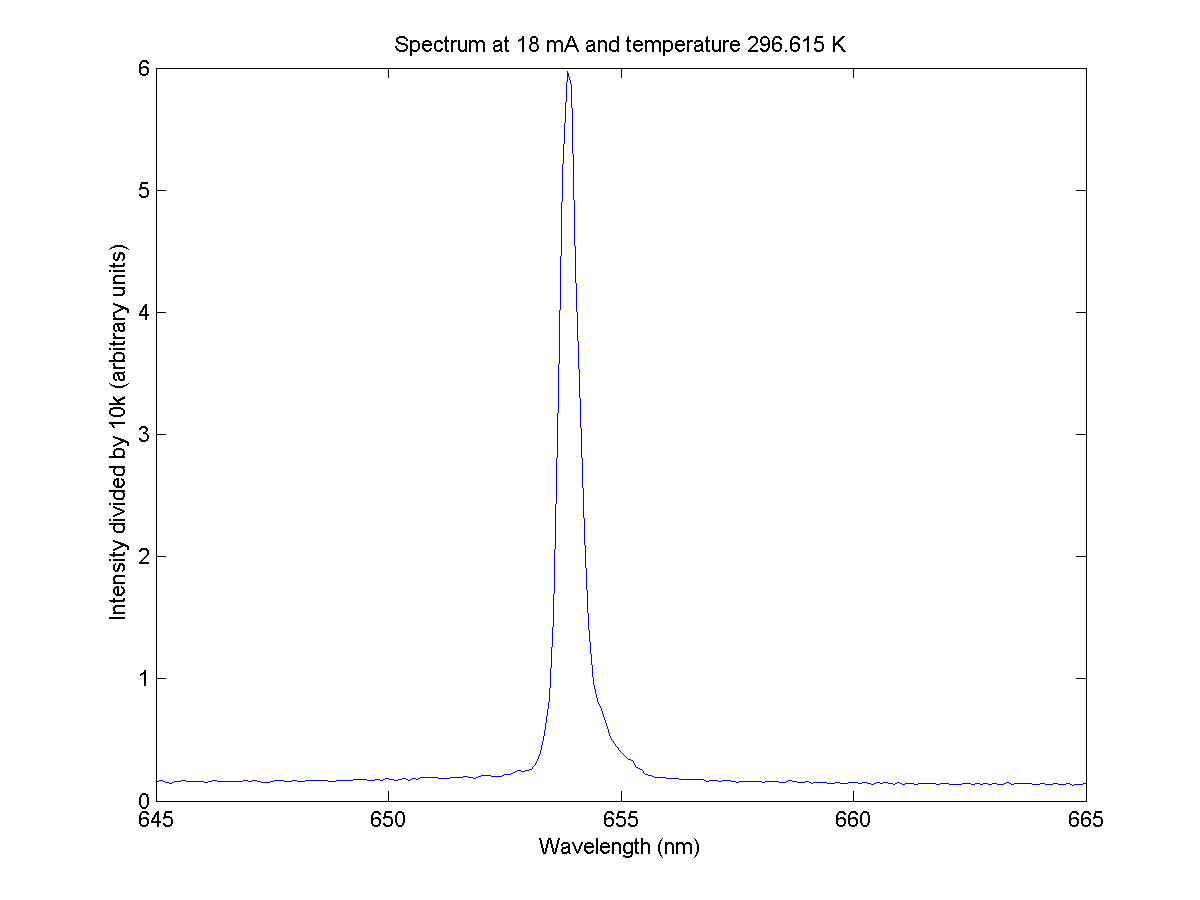
\includegraphics[scale = 0.5]{../Analysis/18mAT10p643.png}
\end{figure}
Our observations are recorded in Tables 3 and 4, and described graphically in Figures 6 and 7.
\begin{table}[H]
\centering
\begin{tabular}{|c|c|}
\hline
Current (mA) & Wavelength (nm) at Fixed Temperature 299.8 K\\
\hline
19 & 655 \\
\hline
18 & 655 \\
\hline
17 & 655 \\
\hline
\end{tabular} 
\caption{Current dependence of peak mode at fixed temperature.}
\end{table}
\begin{table}[H]
\centering
\begin{tabular}{|c|c|}
\hline
Temperature (K) & Wavelength (nm) at Fixed Current 18 mA\\
\hline
300.1 & 655 \\
\hline
299.8 & 655 \\
\hline
298.0 & 654.6 \\
\hline
295.8 & 654.1 \\
\hline
\end{tabular} 
\caption{Current dependence of peak mode at fixed current.}
\end{table}
\begin{figure}[H]
\centering
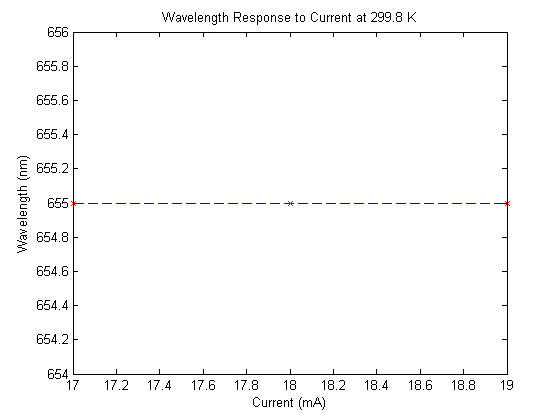
\includegraphics[scale = 0.8]{../Analysis/wavelength-current.png}
\caption{Slope = 0 nm/mA}
\end{figure} 
\begin{figure}[H]
\centering
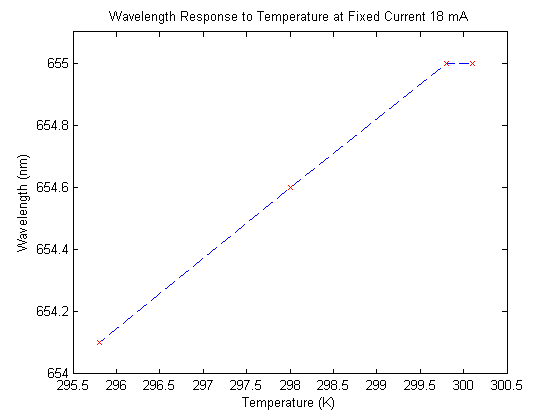
\includegraphics[scale = 0.8]{../Analysis/wavelength-temperature.png}
\caption{Slope = 0.22 nm/K selectively}
\end{figure}
\noindent At this juncture, we should note that there was significant mode-hopping occurring at 295 and 298 K for 18 mA. Measurements recorded there are therefore only approximate.
\section*{Part 2: Creating an External Cavity Diode Laser}
We now built an external cavity diode laser by placing a diffraction grating in the beam's path, and aimed a diffraction mode back into the laser. By the time we did this portion of the experiment, most of the diffraction gratings had been ruined, forcing us to use the only available one in this lab. Our background corrections was about 23 mV with the lights off.\\
\\
The original laser beam power, prior to diffraction, was measured to be 4.34 volts (1.4 mW) on the photodiode. After diffraction, \textbf{three} significant orders could be identified. The leftmost (in the direction facing away from the photodiode) first order mode carried a power of 357 mV (0.12 mW); the retro-reflected central order mode carried a power of 177 mV (0.05 mW); the rightmost first order mode carried a power of 3.33 V (1.11 mW). This odd distribution of powers is currently not within our power to explain.\\
\\
At this juncture, we attempted to aim the rightmost first-order beam back into the laser diode. After some twenty minutes of labour, we succeeded in optimising power output from the first order mode - where originally the power output had fallen to 135 mV (0.04 mW) for the first mode, after optimisation it rested at a much healthier 185 mV (0.06 mW).\\
\\
Using the same methods employed in Part 1, we identified the threshold current to be at \textbf{16.44} mV. This value was determined solely by using the cursor on the oscilloscope; while raw data was downloaded, they appear to be incomplete datasets on my computer, containing either Channel 1 vs. time or Channel 2 vs. time but not both for the same measurement. This is probably a human error.

\subsection*{Measuring Spectrum Dependence on Temperature and Current}

We essentially repeated our experiments in Part 1 for temperature and current dependence immediately afterward.\\
\\
\textbf{No raw data plots are available owing to significant, rapid mode hopping for every iteration}. The Ocean Optics software we used could not save the spectrum at the same rate at which the laser diode kept jumping between modes. This erratic behaviour also significantly affected the quality of our measurements for peak wavelength, and thus we can offer only approximations. For each mode-hopping sample, we attempted to determine a rough running average of the peak wavelength for a full period of about ten seconds. 
\begin{figure}[H]
\centering
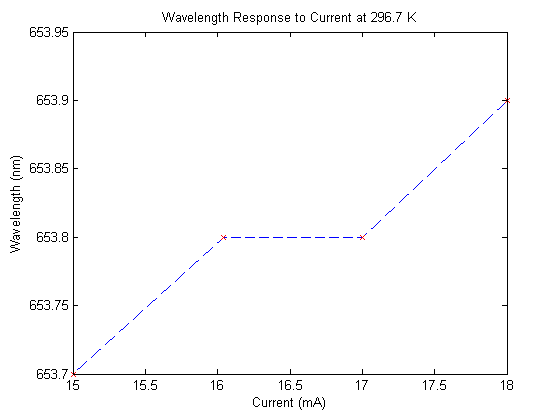
\includegraphics[scale=0.7]{../Analysis/diff_wave_currents.png}
\caption{Slope = 0.0654 nm/mA on average} 
\end{figure}
\begin{figure}[H]
\centering
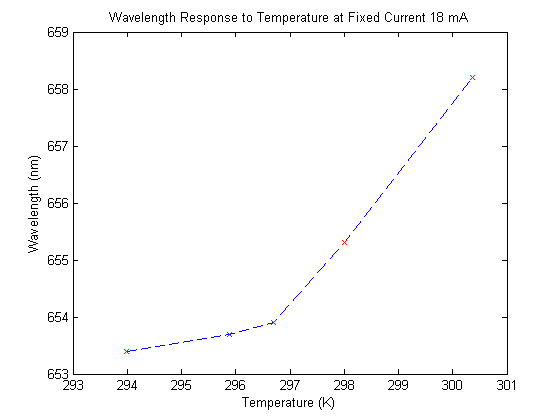
\includegraphics[scale=0.7]{../Analysis/diff_wave_temperatures.png}
\caption{Slope = 0.6765 nm/K on average} 
\end{figure}
\noindent We next measured how much the wavelength changed per unit of rotation of the horizontal adjust of the diffraction grating. Given that 1 complete twist of the knob results in about 8 mrad of a degree shift, we find that turning the knob by 1/16th of a twist (i.e. by 0.5 mrad), we were able to see modes at 657.9, 655.6 and 654.6. In other words, \textbf{a 0.5 mrad shift allowed us to see a wavelength change of about 3.3 nm} - this very roughly corresponds to my calculated 7 nm wavelength shift for a degree shift of about 1 mrad. Please note that there was again significant mode-hopping occluding the experiment.\\
\\
Finally, we attached a piezodrive to the horizontal adjust and drove it at about 0.5 Hertz, at an offset of 5 V, for a peak-to-peak voltage of 6.1 V. Due to the rapid nature of this measurement, we qualitatively record our observations as observing modes at 655.6 nm alternate with modes at 657.9 nm every second. 
\end{document}